\subsection{Test Cross Origin Resource Sharing - OTG-CLIENT-007}
\begin{longtable}[l]{ p{2.3cm} | p{.79\linewidth} }\hline
    & \textbf{Online Banking}
    \\ \hline
    \textbf{Observation} & It was found that Cross Origin Resource Sharing is not possible since the \code{Access-Control-Allow-Origin} header was not set in the requests and hence the application does not support cross origin requests. \\
    \textbf{Discovery} &
        Though a Javascript code snippet was written to test for CORS support, we were not able to simulate cross site requests directly. Refer \ref{code:test_cors} for the code snippet.
        Hence we used the \enquote{test-cors.org} website to make a request to the application and it failed with the error that the header \code{Access-Control-Allow-Origin} was missing. See Figure \ref{fig:test_cors}. The header should have been set to * or some domain in order to serve cross domain requests.
    \\
    \textbf{Likelihood} & N/A \\
    \textbf{Impact} & N/A \\
    \textbf{Recommen\-dations} & N/A \\ \hline
    \textbf{CVSS} & N/A
    \\ \hline
\end{longtable}

\begin{longtable}[l]{ p{2.3cm} | p{.79\linewidth} }\hline
    & \textbf{SecureBank}
    \\ \hline
    \textbf{Observation} & It was found that Cross Origin Resource Sharing is not possible since the \code{Access-Control-Allow-Origin} header was not set in the requests and hence the application does not support cross origin requests. \\
    \textbf{Discovery} & Same as described for Online Banking. \\
    \textbf{Likelihood} & N/A \\
    \textbf{Impact} & N/A \\
    \textbf{Recommen\-dations} & N/A \\ \hline
    \textbf{CVSS} & N/A
    \\ \hline
\end{longtable}

\subsubsection{Comparison}
Neither of the applications support cross domain requests and hence this vulnerability does not exist.

\begin{lstlisting}[caption={Javascript code for testing CORS support}\label{code:test_cors}, language=PHP, basicstyle=\footnotesize, frame=single, captionpos=t, linewidth=.9\textwidth, xleftmargin=.12\textwidth]
    function createCORSRequest(method, url){
        var xhr = new XMLHttpRequest();
        if ("withCredentials" in xhr){
            xhr.open(method, url, true);
        } else if (typeof XDomainRequest != "undefined"){
            // IE8 and IE9
            xhr = new XDomainRequest();
            xhr.open(method, url);
        } else {
            xhr = null;
        }
        return xhr;
    }

    var request = createCORSRequest("get", "<IP-address/secure
        -coding/public/login.php>");
    if (request){
        request.onload = function(){
            //use request.responseText and handle success
        };
        request.onerror = function() {
          // error handling
        }
        request.send();
    }
\end{lstlisting}


\begin{figure}[ht]
	\centering
		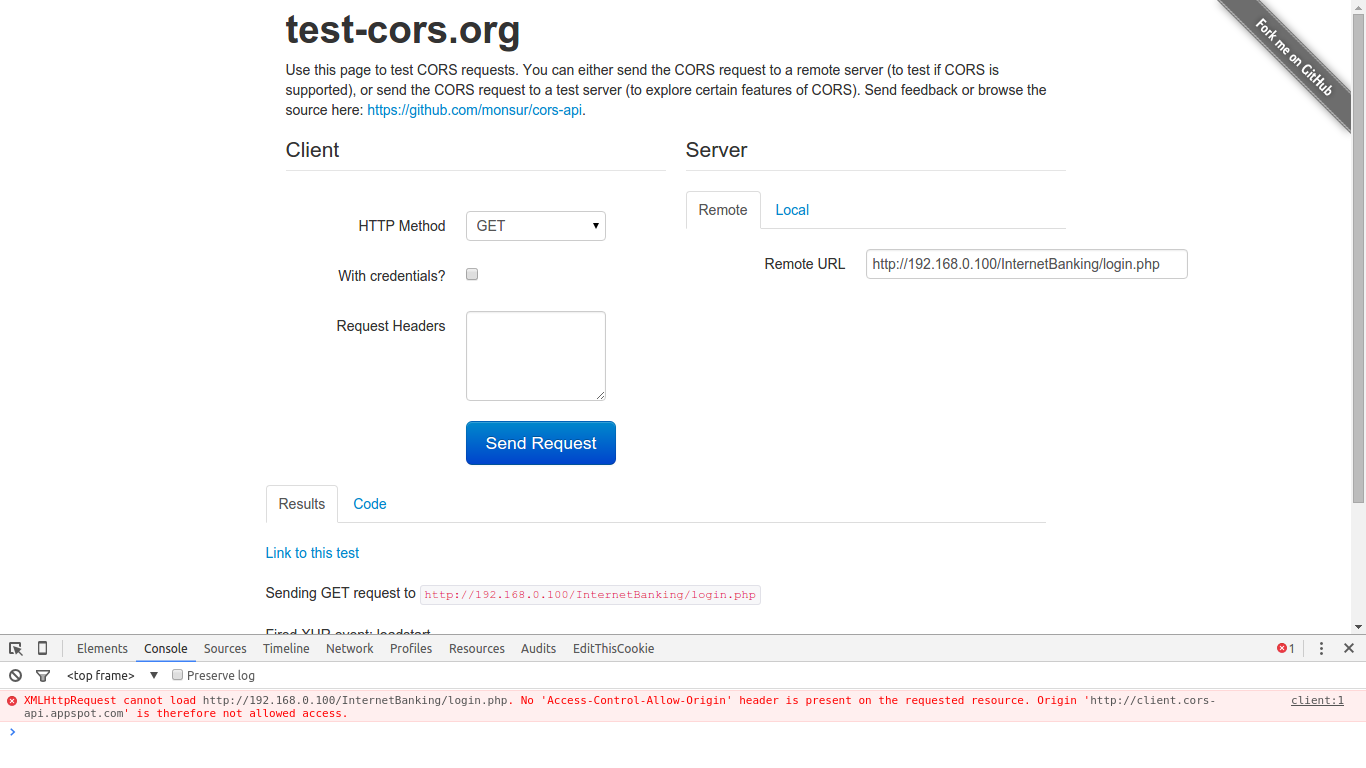
\includegraphics[width=.8\linewidth]{figures/OTG-CLIENT-007.png}
		\caption{Test for Cross Origin Resource Sharing}
	\label{fig:test_cors}
\end{figure}

\clearpage